\documentclass{article}
\usepackage{graphicx} % Required for inserting images
\usepackage{quantikz}
\usepackage{physics}
\usepackage{amssymb}
\usepackage[margin = 2cm]{geometry} 
\usepackage{hyperref}
\usepackage{minted}

\usepackage{quantikz}

\begin{document}

\noindent {\Huge \textbf{$\hat Q\ket{B}$asics}}\\
{\large \textbf{Activity 4:} Characterizing quantum states \\

\section*{Ramsey Fringe}
Suppose you are given a quantum gate $U(\theta)$ for some unknown $-\frac{\pi}{2} < \theta < \frac{\pi}{2}$ (*\textit{correction: should say $0 \leq \theta < \pi$}) which maps $\ket{0}$ to $\ket{\theta} = \frac{1}{\sqrt{2}}(\ket{0}+e^{i\theta}\ket{1})$. You can run the quantum circuit as many times as you want. Using a Hadamard gate and $Z-$basis measurements, how can you determine $\theta$? Try it out in Qiskit.

\subsection*{Solution}
In rough terms, a Hadamard gate converts relative phase between the two basis states $\ket{0}$ and $\ket{1}$ in superposition into a difference in amplitudes. This corresponds to switching the measurement basis from $Z$ to $X$. Recall that $H \ket{0} = \ket{+}$ and $H \ket{1} = \ket{-}$, where
\begin{align*}
\ket{+} &= \frac{\ket{0} + \ket{1}}{\sqrt{2}} & \ket{-} &= \frac{\ket{0} - \ket{1}}{\sqrt{2}}
\end{align*}
We find
\begin{align*}
H\ket{\theta} &= \frac{\ket{+}+ e^{i\theta}\ket{-}}{\sqrt{2}} \\
&= \frac{1}{2}\qty((1+e^{i\theta})\ket{0} + (1-e^{i\theta})\ket{1}) \\
&= e^{i\theta/2}\left(\left(\frac{e^{i\theta/2}+ e^{-i\theta/2}}{2}\right)\ket{0} + \left(\frac{e^{i\theta/2}-e^{-i\theta/2}}{2}\right)\ket{1}\right) \\
&= e^{i\theta/2}(\cos(\theta/2)\ket{0} + i\sin(\theta/2)\ket{1})
\end{align*}
Therefore we measure $\ket{0}$ with probability $\cos[2](\theta/2) = \frac{\cos(\theta)+1}{2}$. In order to determine $\theta$ experimentally, we run the circuit many times and compute the fraction of time $\ket{0}$ is measured and solve for $\theta$. This recovers $\theta$ uniquely if $0 \leq \theta < \pi$. In order to fully recover theta, we need another set of measurements, which the next question will establish. Here is the code to run this in Qiskit:
\begin{minted}{python}
from qiskit import QuantumCircuit, execute
from qiskit.providers.aer import AerSimulator
from matplotlib import pyplot as plt
import numpy as np
sim = AerSimulator()
def prep(theta):
    qc = QuantumCircuit(1)
    #prepare |theta>
    qc.h(0)
    qc.rz(theta, 0)
    return qc
thetas = np.linspace(0, np.pi-.01, 100)
theta_guesses = []
shots = 1000 #precision
for theta in thetas:
    qc = prep(theta)
    qc.h(0)
    qc.measure_all()
    counts = execute(qc, sim, shots = shots).result().get_counts().get("0",0)
    expfreq = counts/shots
    theta_guesses.append(np.arccos(2*expfreq - 1))
np.nan_to_num(theta_guesses);
\end{minted}
\begin{centering}
    \begin{figure}[hbt!]
        \centering
        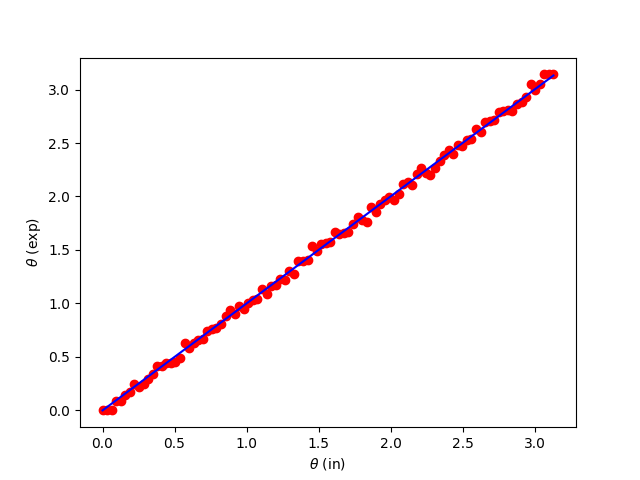
\includegraphics[width = .6\textwidth]{RamseyFringe.png}
        \label{fig:enter-label}
    \end{figure}
\end{centering}
\subsection*{Solution 2}
With a little more machinery, there is a more illuminating way to solve this problem. By the Pauli-Euler identity,
$$
\ket{\theta} = e^{i\theta \frac{Z+1}{2}}\ket{+} = e^{i\frac{\theta}{2}}e^{i\frac{\theta}{2}Z}\ket{+} = e^{i\frac{\theta}{2}}e^{i\frac{\theta}{2}Z}H\ket{0}
$$
Since $HZH = X$, we have $He^{i\frac{\theta}{2} Z}H = e^{i\frac{\theta}{2} X}$ (which you can see by considering the Taylor series), and so
$$
H\ket{\theta} = e^{i\frac{\theta}{2}}He^{i\frac{\theta}{2} Z}H\ket{0} =  e^{i\frac{\theta}{2}}e^{i\frac{\theta}{2} X}\ket{0}
$$
Using the Pauli-Euler identity again,
$$
 e^{i\frac{\theta}{2}}e^{i\frac{\theta}{2} X}\ket{0} =  e^{i\frac{\theta}{2}}(\cos(\frac{\theta}{2})\ket{0} + i\sin(\frac{\theta}{2})\ket{1})
$$
which gives the same result as above.
\section*{The Bloch Sphere}
The $X$, $Y$, and $Z$ operators are related to the $\hat x$, $\hat y$, $\hat z$ axes, and now we are in a position to explore this connection. Let
$$
\ket{\theta, \phi} = \cos(\theta/2)\ket{0} + \sin(\theta/2)e^{i\phi}\ket{1}
$$
As a reminder, the outer product definitions of $X,Y,$ and $Z$ are
\begin{align*}
X &= \ketbra{0}{1} + \ketbra{1}{0} & Y &= -i\ketbra{0}{1} + i\ketbra{1}{0} & Z &= \ketbra{0}{0} - \ketbra{1}{1}
\end{align*}
\subsection*{Part a}
Show that
\begin{align*}
\langle X \rangle &= \sin(\theta)\cos(\phi) \\
\langle Y \rangle &= \sin(\theta)\sin(\phi) \\
\langle Z \rangle &= \cos(\theta)
\end{align*}
This is the polar representation of a vector on the unit sphere. In this representation, the $X-$eigenkets $\ket{+}, \ket{-}$ (corresponding to $\theta = \pm\pi/2$ and $\phi = 0$) lie on the $\hat x-$axis, the $Y-$eigenkets $\ket{i},\ket{-i}$ (corresponding to $\theta = \pm\pi/2$ and $\phi = \pi/2$) lie on the $\hat y-$axis, and the $Z-$eigenkets $\ket{0},\ket{1}$ (corresponding to $\theta = 0, \pi$) lie on the $\hat z-$axis.

\subsection*{Solution}
We have shown previously that if $\ket{\psi} = \alpha \ket{0} + \beta \ket{0}$ then
\begin{align*}
    \langle Z \rangle &= |\alpha|^2 - |\beta|^2 \\
    \langle Y \rangle &= 2\Im(\alpha^\ast \beta) \\
    \langle X \rangle &= 2\Re(\alpha^\ast \beta)
\end{align*}
Applying this to $\ket{\theta, \phi}$, we find
$$
\langle Z \rangle = \cos[2](\theta/2) - \sin[2](\theta/2) = \cos(\theta)
$$
$$
\langle Y \rangle = 2\Im(\cos(\theta/2)\sin(\theta/2)e^{i\phi}) = 2\cos(\theta/2)\sin(\theta/2)\Im(e^{i\phi}) = \sin(\theta)\sin(\phi)
$$
$$
\langle X \rangle = 2\Re(\cos(\theta/2)\sin(\theta/2)e^{i\phi}) = 2\cos(\theta/2)\sin(\theta/2)\Re(e^{i\phi}) = \sin(\theta)\cos(\phi)
$$
\subsection*{Part b}
\par Now let $\hat n = (\langle X \rangle, \langle Y \rangle, \langle Z \rangle)$. 
Show that
$$
\ketbra{\theta, \phi}{\theta, \phi} = \frac{I + n_xX + n_yY + n_zZ}{2}
$$
The vector $\hat n$ is often called the Bloch vector of the state $\ket{\theta, \phi}$.

\subsection*{Solution}
Foiling out the outer product,
\begin{align*}
\ketbra{\theta, \phi}{\theta, \phi} &= \mqty(\cos(\theta/2) \\ e^{i\phi}\sin(\theta/2)) \mqty(\cos(\theta/2) & e^{-i\phi}\sin(\theta/2))\\
&= \mqty(\cos(\theta/2)\cos(\theta/2) & e^{-i\phi}\cos(\theta/2)\sin(\theta/2) \\ e^{i\phi}\cos(\theta/2)\sin(\theta/2) & \sin(\theta/2)\sin(\theta/2)) \\
&= \frac{1}{2}\mqty(1+\cos(\theta) & \sin(\theta)e^{-i\phi} \\ \sin(\theta)e^{i\phi} & 1-\cos(\theta)) \\
&= \frac{1}{2}\mqty(1+n_z & n_x - in_y \\ n_x + i n_y & 1-n_z) = \frac{1}{2}\mqty(1 & 0 \\ 0 & 1) + \frac{n_x}{2}\mqty(0 & 1 \\ 1 & 0) + \frac{n_y}{2}\mqty(0 & -i \\ i & 0) + \frac{n_z}{2}\mqty(1 & 0 \\ 0 & -1)
\end{align*}
This gives the desired result. The outer product $\ketbra{\theta, \phi}{\theta, \phi}$ is commonly known as the density matrix.
\end{document}
